\chapter{Experiments}
In this chapter, we provide details on the techniques used to gather the data presented in the previous chapter. We also present additional experimental results.


\section{SSD training}
\citeauthor{bib:ssd} implemented \footnote{\url{https://github.com/weiliu89/caffe/tree/ssd}} SSD model from their research paper in the \textit{Caffe} \footnote{\url{http://caffe.berkeleyvision.org/}} deep learning framework. We decided against performing our experiments in this, by now outdated framework, and implemented our version in newer \textit{PyTorch} \footnote{\url{https://pytorch.org/}} framework (more detailed technical specification of used libraries is available in \cref{app:impl}).

We started by implementing a common framework for SSD detectors, that would support SSD models with many modifications. Although SSDTC inference is possible in the same framework, we had to create a separate environment for the training (more on SSDTC in \cref{sec:ssdtcImpl}). 

The main characteristics of our framework are the use of \textit{SGD} optimizer and the loss function defined for SSD, also called MultiBox loss (\cref{sec:ssd}). Another essential element of the detection pipeline, used for inference, is the non-maximum suppression algorithm. The parametrization of these modules can be seen in \cref{tab:trainParams}. It is also worth mentioning that for the sake of consistency, all experimental models were trained for 401 epochs with a batch size of 32, using those default parameters.

\begin{table}
    \centering
    \begin{tabular}{c c|c c| c c}
        \multicolumn{2}{c|}{MultiBox loss} & \multicolumn{2}{c|}{SGD optimizer} & \multicolumn{2}{c}{NMS} \\
        \hline
        IoU threshold & 0.5 & learning rate &  \num{e-3} & IoU threshold & 0.5\\
        \hline
        \multirowcell{2}{positive/negative\\ sample ratio} & \multirowcell{2}{1:3} & \multirowcell{2}{momentum} & \multirowcell{2}{0.9} & \multirowcell{2}{confidence \\ threshold} & \multirowcell{2}{0.2} \\
        & & & & & \\
        \hline
        & & weight decay & \num{5e-4} & & \\
    \end{tabular}
    \caption{A selection of default values for most important parameters in our framework. We used these values for training and evaluation in all experiments. Note that the learning rate decreases during the training.}
    \label{tab:trainParams}
\end{table}


\section{Measurements}
To make our work comparable to other similar studies and future works, we explain methods used for both precision and performance measurements.

\subsection{Precision}
Rather than implementing a copy of the precision evaluation, our precision measurements were taken using an external tool. Using the external tool, independent on our implementation, allows us to easily compare our results with other works with little to no modifications. We used the implementation by \citet{bib:metricsgit} that mirrors the evaluation process of the PASCAL VOC Challenge. The test setup used default parameters, meaning that the interpolation of AP was calculated using all data points and the IoU threshold was set to 0.5. 

We present all the measurements taken on Surveillance dataset while performing multiple experiments described in this thesis in \cref{tab:ap}.


\begin{table}
    \centering
    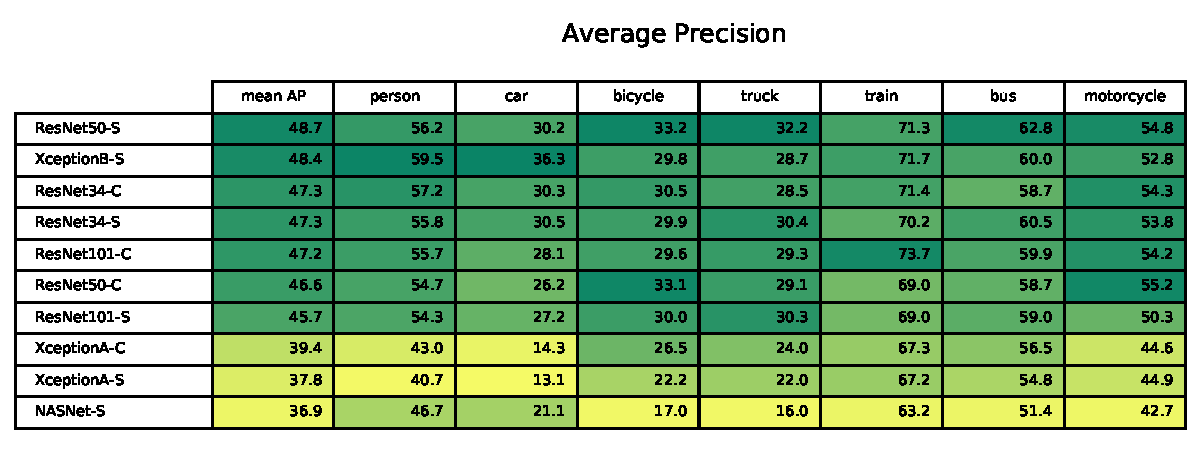
\includegraphics[width=\textwidth]{img/ap}
    \caption[Average precision of all tested networks on Surveillance classes]{Average precision of all tested networks on Surveillance classes. COCO indicates that the network was trained on COCO dataset, otherwise only Surveillance data were used for training.} 
    \label{tab:ap}
\end{table}

\subsection{Inference speed}
The absolute values of the inference speed measurement would not provide any information without the knowledge of the environment in which they have been taken. In this section, we provide the details of both software and hardware environments used for measurements.

Testing was done by processing a total of 10 000 images in batches of 16. This process was timed, and the average \textit{fps} value was calculated.  Since we do not consider scaling and cropping the images to be part of the network, we did not need to include this process in the measurement. The set of [300\x300] pixel images was pre-loaded into memory before the timer was started. On the other hand, non-maximum suppression is a critical part of the algorithm and is included in the measurement. 

\paragraph{}
\noindent All our testing was done on the following hardware:
\begin{itemize}
    \item AMD EPYC 7401P CPU @ 2GHz \x 24
    \item NVIDIA GeForce GTX 1080 Ti
    \item 128GB DDR4 RAM
\end{itemize}


\section{Improving the Xception-SSD}
In \cref{sec:fixxception} we introduced a hypothesis about Xception\textit{A}-SSD. Based on this hypothesis, we presented the improved Xception\textit{H} model. However, as suggested by the name, it was not our first modification, and we needed some trial-and-error testing to achieve this result.

We will describe every iteration of the Xception-SSD model we trained and the reasoning behind the particular modifications. For clarity, we will refer to the Xception\textit{X} models in this section only by their version letters. The performance of mentioned models on Surveillance dataset is plotted on \cref{fig:xception_perf}, and more details on precision in \cref{tab:ap}. Also, the feature map sizes inside the models are shown in \cref{tab:xmods}.


\begin{figure}
    \centering
    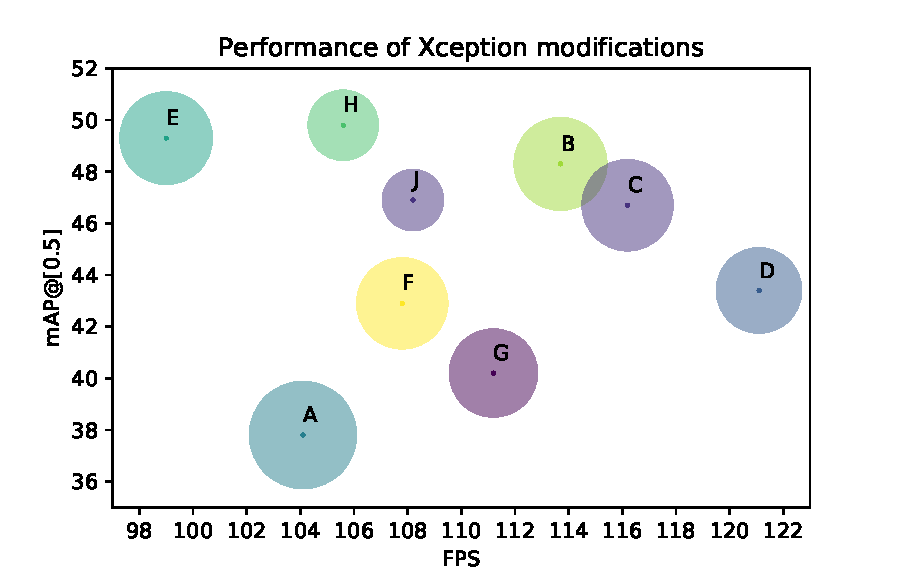
\includegraphics[width=0.95\textwidth]{img/fps_map_x}
    \caption[Performance of multiple Xception modification on Surveillance dataset]{Performance of multiple Xception modification on Surveillance dataset. Circle radii demonstrate relative difference of network parameter counts.} 
    \label{fig:xception_perf}
\end{figure}

\begin{table}
    \centering
    \begin{tabular}{c|c|c|c|c|c}
            &   A   &   B (C, D)   &   E (F, G)   &   H   &   J   \\
        \hline
        B1  &   [74\x128]   &   [74\x128]   &   [74\x128]   &   [74\x128]   &   [74\x128]   \\
        B2  &   \textbf{[37\x256]}   &  [37\x256]   &   [37\x256]   &   [37\x256]   &   [37\x256]   \\
        B3  &   [19\x728]   &   [19\x256]   &   [37\x256]   &   [37\x256]   &   [37\x256] \\
        \hline
        B4-6  &   [19\x728]   &   [19\x256]   &   [37\x256]   &   [37\x256]   &   [37\x256] \\
        B7  &   [19\x728]   &   \textbf{[19\x256]}   &   \textbf{[37\x256]}   &   \textbf{[37\x256]}   &   \textbf{[37\x256]} \\
        B8-10  &   [19\x728]   &   [19\x728]   &   [19\x728]   &   [19\x512]   &   [19\x512]\\
        B11 &   \textbf{[19\x728]}   &   \textbf{[19\x728]}   &   \textbf{[19\x728]}   &   \textbf{[19\x512]}   &   \textbf{[19\x512]}\\
        \hline
        B12 &   [10\x1024]  &   [10\x1024]  &   [10\x1024]  &   [10\x728]  &   [10\x512]\\
        S1  &   [10\x1536]  &   [10\x1536]  &   [10\x1536]  &   [10\x1024]  &   [10\x512]\\
        S2  &   \textbf{[10\x2048]}  &   \textbf{[10\x2048]}  &  \textbf{[10\x2048]}   &  \textbf{[10\x1024]} &  \textbf{[10\x512]}\\
    \end{tabular}
    \caption{A table of feature map sizes on the output of layers of the Xception networks. Bx stand for Xception blocks, S1 and S2 stand for separable convolution layers that follow the block structure (see \cref{fig:xception}). The first number represents spatial dimensions of a square feature, expecting [300\x300] input, and the second one represents the number of channels. The highlighted feature maps are used for the detections. The versions C, D, and F, G share the feature maps sizes with their parent versions, if the given layers are present, but do not match the highlighted feature extraction.}
    \label{tab:xmods}
\end{table}

\subsubsection{Versions B, C, D}
We examine this trio at once,  since version \textit{C} adds modifications to version \textit{B}, and version \textit{D} further modifies version \textit{C}. Notably, we trained these models in parallel and therefore had no results from concurrent models to inform on the design.

Starting with the assumption that the problem of the version \textit{A} is the position of the first feature extraction for detection, we moved the extraction from \textit{block 2} to \textit{block 7}. We also reduced the number of output filters on \textit{blocks 2 to 7} from 728 to 256. As a result, the first detection is performed on a [19\x19\x256] feature map as opposed to the [37\x37\x256] map of \textit{A}. The main factor here, it that the feature map is extracted after the data pass five additional blocks. 

Due to a reduction of feature map size, we considered this modification a half-measure in our plan to move the first feature extraction deeper into the network. However, it proved to be a successful step in the right direction. The network has significantly gained in both speed and precision values. 

Both versions \textit{C} and \textit{D} were designed for observation of the impact of the removal of parts of the network. We designed the modifications in such a way that they would not affect other layers. For clarity, the removals of blocks and layers do not alter the numbering scheme.

Version \textit{C} omits \textit{blocks 5, 6 and 7} and extracts the [19\x19] feature map after \textit{block 10} instead of \textit{block 11}. However, we did not observe a satisfying performance boost to justify received loss of precision. 

Version \textit{D} was designed to test the need for six detection layers, mainly the layers for detecting large objects. It is based on \textit{C} and removes the feature layers produced by \textit{extra layers}. Although the observed performance boost from \textit{C} to \textit{D} was more significant than the one from \textit{B} to \textit{C},  it was also coupled with a major precision penalty.

\subsubsection{Versions E, F, G}
Similarly to the previous trio, these versions are also based on each other, with the main architectural change being applied in \textit{E}. Versions \textit{F} and \textit{G} were designed to perform independent experiments. 

Version \textit{E} is the one, where we finally implemented our original intention of moving the first extracted feature map of [37\x37] size to a deeper layer. Implementation-wise, the only difference between \textit{B} and \textit{E}, is the removal of max-pooling with stride 2 from \textit{block 2} and placing it to \textit{block 8}. This movement results in the increase of feature size to the desired [37\x37] map up to \textit{block 8}.

We observed a noticeable drop-off in performance compared to version \textit{B} and a slight increase in precision. Although the number of parameters in the network is the same, the change from [19\x19] to [37\x37] requires about four times more computation per convolutional layer.

Version \textit{F} modifies \textit{E} in the same way, \textit{C} modified \textit{B}. It skips the \textit{blocks 5, 6 and 7} and extracts the second feature map after \textit{block 10}. Although the received performance boost in relation to \textit{E} is significant, the precision is also significantly impacted in a negative way.

Version \textit{G} repeated the experiment from version \textit{D}, but instead of removing the last three detection feature maps, we removed every other one, thus keeping the first, third and fifth ones. It is based on version \textit{F}, and again we see the precision loss we cannot justify by performance gain.

\subsubsection{Version H}
Since we managed to gain the best precision result with version \textit{E}, we decided to try and increase its performance. To this end, we designed the version \textit{H}. However, tests \textit{C},\textit{F}, \textit{D} and \textit{G} showed that the removal of blocks or detection layers from the network is detrimental for the result. Therefore we decided for a less radical solution of trimming the channel depth of the network. We ended up trimming the [19\x19] feature map to 512 channels and [10\x10] map to 1024 channels.

Experiments show that this adjustment not only put the performance of the model halfway between \textit{E} and \textit{B} but also slightly boosted the precision.

\subsubsection{Version J}
After the success of version \textit{H}, we decided to try the limits of channel removal approach. We started with the setup of \textit{H}, and set the number of channels of every layer following \textit{block 7} up to \textit{extra layers}, to 512. 

Version \textit{J}, showed us, that this is also not a viable solution. The results are underwhelming in both, precision and performance.


\subsubsection{Conclusion}
In conclusion, we managed to receive the best precision results from the version \textit{H}. Our first implementation, \textit{A}, managed only 37.8\% mAP on Surveillance dataset. Meanwhile version \textit{H} achieved 49.8\% mA on the same data while keeping the performance equivalent.

\section{SSDTC implementation and training}
\label{sec:ssdtcImpl}
We have already described the architecture of SSDTC in \cref{sec:ssdtc}; however, the actual implementation and training process proved to be more complicated than SSD. In this section, we go through the challenges brought by SSDTC. 

As mentioned, we based the SSDTC on ResnNet34-SSD. We used the SSD initialized by the weights we learned on Surveillance dataset. We did not need the detection layers of SSD, so we removed them from the model. The resulting ResNet34 with \textit{extra layers} served as a feature extractor for both SSDTC and also for training the baseline SSD on HollywoodHeads dataset. For training of both networks, we froze the weights in the extractor and trained only temporal and detection layers. It is important to note that every image processed by SSDTC, passes through the same extractor. 

The SSDTC design we created, has different input data requirements for training and inference. To properly train, it needs a large number of smallest possible chunks in a batch for the network. However, one large chunk is the most effective way for inference and the most natural way as we expect a continuous video stream.

This, however, poses conflicting requirements for the implementation of the network, namely in the passing of data between the modules. For the purposes of explanation, lets call the ResNet34 network with \textit{extra} layers the \textit{Extractor}, the two conv3d layers the \textit{Temporal module}, and the localization and classification layers the \textit{Detection module}. We will also consider the detection process for only one of six feature map layers of the Extractor. 

During training, the network starts with feature extraction on seemingly independent \textit{n*c} frames in a batch (\textit{c} being the minimal possible chunk, in our case 5, and \textit{n} the batch size). Coming to the temporal layers, the feature maps need to be reshaped to represent \textit{n} chunks of size \textit{c} to allow for conv3d layers. After the temporal layers, the feature maps come out in the batch size of \textit{n}, but due to the nature of temporal layers, the chunk size is reduced to 1. This data then has to be reshaped again, to remove the temporal dimension, and create a batch of size \textit{n} for the detection layers.  

On the other hand, during inference, the input is a single chunk of consecutive frames, that is equivalent to a single batch. This batch can be simply passed thorough feature extraction layers, and the only modification needed for the temporal layers is to encapsulate the whole tensor in additional dimension to represent a temporal batch of size one. After the temporal convolution, we remove the encapsulation and continue with the detection; however, the batch size in this step is smaller than at the beginning. 

We can see the difference between training and inference feature sizes in \cref{tab:ssdtcFeatureSizes}. This behavior forced us into two separate implementations for inference and training. Although both implementations share the same network models, the differences are in the handling of the data between the modules. In the table, we can see that during training, it is the \textit{chunk dimension} that gets eliminated in temporal layers, and during the inference, it is the \textit{batch dimension}. 

Although it is possible to use both versions for training and inference, each has a significant disadvantage if not used as intended. The inference module does not allow for the use of the batch normalization in conv3d layers, because it operates with temporal volume in a batch size one. The fact that the ability to use batch normalization is vital for the training was also experimentally tested. Without normalization, we were not able to over-perform standard SSD with the temporal version. There is a better chance for the training module to be modified for efficient inference, although with some performance hit inherent from our implementation. 

\begin{table}
    \centering
    \begin{tabular}{c|c|c}
        Module &  \multicolumn{2}{c}{Training}\\
        \hline
            & Input   & Output    \\
        Extractor   &  [H$_0$\x W$_0$\x 3\x 5*N] & [H$_1$\x W$_1$\x F$_1$\x 5*N]  \\
        Temporal   &  [H$_1$\x W$_1$\x F$_1$\x 5\x N] & [H$_2$\x W$_2$\x F$_2$\x1\x N] \\
        Detector  &  [H$_2$\x W$_2$\x F$_2$\x N] &      \\
        \hline
        \multicolumn{1}{c}{} & \multicolumn{2}{c}{Inference}\\
         \hline
         & Input   & Output\\
        Extractor   &   [H$_0$\x W$_0$\x 3\x C]  & [H$_1$\x W$_1$\x F$_1$\x C]\\
        Temporal   &  [H$_1$\x W$_1$\x F$_1$\x C\x 1] & [H$_2$\x W$_2$\x F$_2$\x C-4\x 1]\\
        Detector   & [H$_2$\x W$_2$\x F$_2$\x C-4] & \\
        
    \end{tabular}
    \caption{Data shapes and sizes on the input and output of the SSDTC modules. The output of the Detector complies with SSD definitions (\cref{sec:ssd}).}
    \label{tab:ssdtcFeatureSizes}
\end{table}

